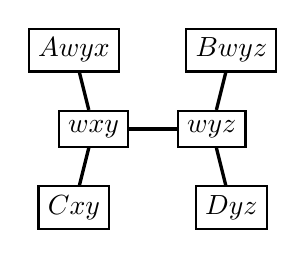
\begin{tikzpicture}
\begin{scope}[every node/.style={rectangle,thick,draw}]
    \node (1) at (-1,1) {$Awyx$};
    \node (2) at (-1,-1) {$Cxy$};
    \node (3) at (-0.75,0) {$wxy$};
    \node (4) at (0.75,0) {$wyz$};
    
    \node (5) at (1,1) {$Bwyz$};
    \node (6) at (1,-1) {$Dyz$};
\end{scope}

\begin{scope}[every node/.style={fill=white,circle},
              every edge/.style={draw=black,very thick}]
    \path [-] (1) edge (3);
    \path [-] (2) edge (3);
    \path [-] (3) edge (4);
    \path [-] (4) edge (5);
    \path [-] (4) edge (6);
\end{scope}
\end{tikzpicture}